\chapter{Technologies \& implémentations}
\label{Chapter3}

Ce chapitre reprend en détail chaque brique, en exposant pour chacune les recherches effectuées et des propositions de solutions pour leur implémentation ou mise en place.

\unsure{déplacer paragraphe ci-dessous ?}
Découvrant les domaines de l'urbanisme et de la modélisation du paysage avec la réalisation de ce projet, j'ai commencé par étudier les technologies et processus les plus répandus dans ces secteurs.
\todo{BIM \& CO ?}

\section{Formats de fichiers 3D}

Dans le cadre de la mise en place d'une plateforme de partage de modèles 3D, l'étude des formats de fichiers existants (usages, tendances, compatibilité...) est un point de départ intéressant. Cela permet tout d'abord de découvrir comment sont représentées les données de modélisation, et comment les manipuler. On prend également connaissance des logiciels principaux du marché.

Au final, cela aidera à décider quel(s) format(s) seraient à considérer pour notre outil, celui-ci devant pouvoir \textbf{supporter les formats les plus courants} afin d'être aisément utilisable.

Il existe plus d'une centaine de formats permettant de stocker des données tridimensionnelles. De nombreuses listes de ces derniers sont disponibles sur internet, mais la plupart ne mentionnent que les principaux formats. La section consacrée à cette catégorie de fichiers sur \textit{Wikipédia}\footnote{\url{https://en.wikipedia.org/wiki/List_of_file_formats\#3D_graphics}} s'avère être l'une des plus fournies. 

\todo{\url{https://www.archives.gov/files/applied-research/ncsa/8-an-overview-of-3d-data-content-file-formats-and-viewers.pdf}}

Cette abondance s'explique entre autres par la variété des domaines concernés : de la représentation de structure moléculaires (format XYZ\footnote{Spécifications du format \textit{XYZ} : \url{http://openbabel.org/wiki/XYZ_\%28format\%29}}), à la cryo-microscopie électronique (format MRC\footnote{Spécifications du format MRC : \url{http://www.ccpem.ac.uk/mrc_format/mrc2014.php}}), en passant par les formats de certains éditeurs de jeux ou consoles (\textit{MDX} chez \textit{Blizzard Entertainment},\textit{BDL} et \textit{BMD3} chez Nintendo...), et bien entendu tous les logiciels de modélisation/animation/CAD (\textit{Blend} pour \textit{Blender}, \textit{FBX}, \textit{MAX}, \textit{MB} et bien d'autres pour les différentes suites proposées par \textit{Autodesk}, \ldots).

Dans le cadre de ce projet, les formats qui nous intéressent sont bien entendu ceux qui concernent l'urbanisme, au travers des logiciels de CAO/DAO correspondants.

Enfin, il est important de savoir qu'un fichier 3D n'est pas qu'une simple liste de coordonnées 3-axes, mais contient généralement de nombreuses informations telles que : 
\begin{itemize}
    \item Caméras : types, emplacements, orientations...
    \item Lumières : types, emplacements, effets...
    \item Maillages (\textit{meshes}),
    \item Textures,
    \item Animations, sons...
\end{itemize}

Le contenu exact varie beaucoup d'un format à l'autre. Aussi, là où un certain format permettra de stocker l'ensemble des informations d'un modèle, un autre nécessitera de séparer les données (par exemple, un fichier pour le squelette, la lumière... et un autre pour les textures). \todo{Exemple concret} 

\todo{section dédiée à ce que contient un fichier 3D ?}

\subsection{Formats de fichiers de DAO/CAO courants}

Les formats les plus présents actuellement sont détaillés ci-après.

\subsubsection{FBX}
\textit{FBX} (\textbf{F}ilm\textbf{b}o\textbf{x}) est un format appartenant à \textit{Autodesk}.

Bien que propriétaire, une \textit{API}\footnote{\url{https://www.autodesk.com/products/fbx/overview}} fournit le nécessaire pour lire et écrire ces fichiers.

Il a été créé pour pallier les variétés de formats rencontrés dans le flux de travail, et ainsi assurer l'interopérabilité entre les produits d'\textit{Autodesk}, tels que \textit{3ds Max}, \textit{Maya} ou \textit{Motion Builder}, ainsi que de nombreux autres logiciels comme \textit{Cinema4D}, \textit{Rhino} ou \textit{Unity3D}.

De fait, cela en fait un format populaire, très répandu.
Une rapide recherche sur \textit{GitHub}\footnote{\url{https://github.com/search?q=fbx+viewer}} nous renvoie de nombreux projets de visionneuses \textit{FBX}.

\subsubsection{COLLADA}
COLLADA (COLLAborative Design Activity) is an interchange file format for interactive 3D applications. It is managed by the nonprofit technology consortium, the Khronos Group, and has been adopted by ISO as a publicly available specification, ISO/PAS 17506.

COLLADA defines an open standard XML schema for exchanging digital assets among various graphics software applications that might otherwise store their assets in incompatible file formats. COLLADA documents that describe digital assets are XML files, usually identified with a .dae (digital asset exchange) filename extension. [Source : Wikipedia]

Advantages : maintained by a non profit consortium, ISO, spec publicly available. Open Standard..
Disadvantages : seems not widely represented : e.g. not many projects of DAE viewers on GitHub

Default format for importing/exporting models in Blender software

\subsection{3ds}


\subsubsection{glTF}
\label{sec:glTF}


glTF (GL Transmission Format)\footnote{\url{https://www.khronos.org/gltf/}} is a file format for 3D scenes and models using the JSON standard. It is described by its creators as the "JPEG of 3D." It is an API-neutral runtime asset delivery format developed by the Khronos Group 3D Formats Working Group. [Source : Wikipedia]

sketchfab gltf description and models

Sketchfab provides an autoconverted version in gLTF format for all downloadable models.

\subsection{Logiciels et compatibilité}


\section{Building Information Modeling (BIM)}

\begin{figure}
    \centering
    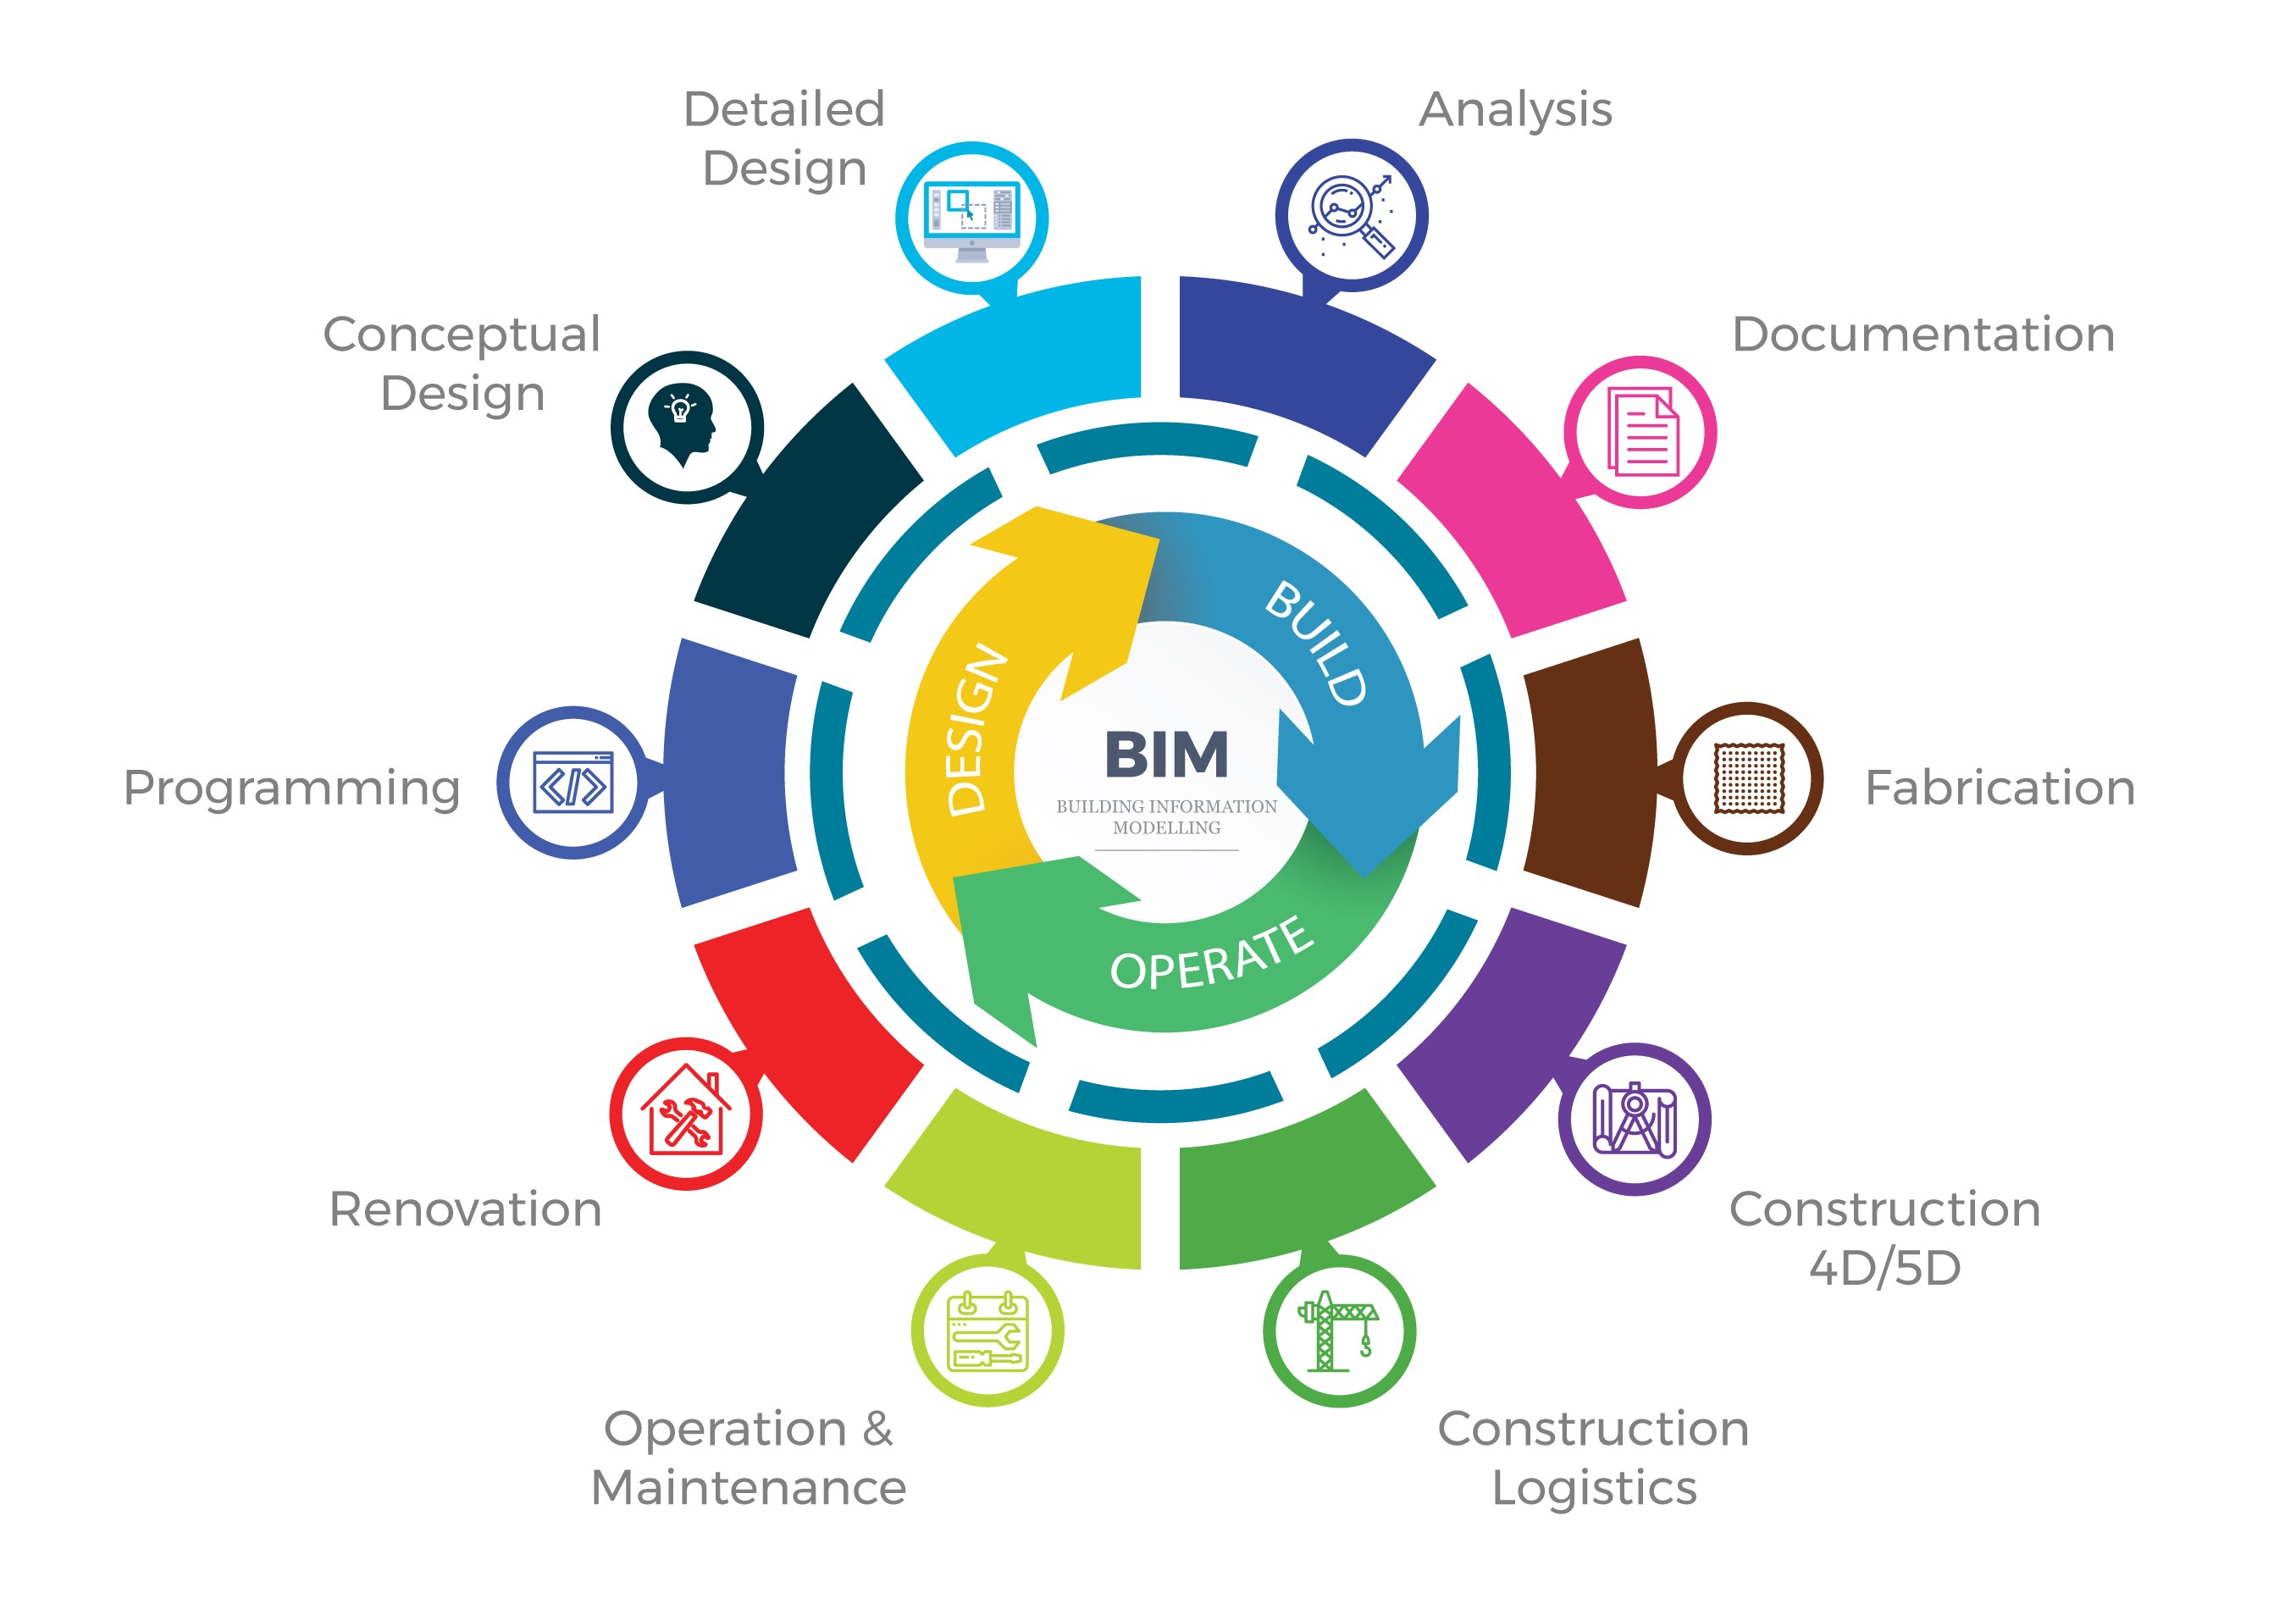
\includegraphics[width=\linewidth]{Figures/bim-process.jpg}
    \caption{Processus BIM}
    \label{fig:bim-process}
\end{figure}

\url{http://objectif-bim.com/index.php/openbim/bcf-format-de-collaboration-bim}

\url{http://njhcadservices.co.uk/?page_id=32}

\section{Système d'information géographique (SIG)}
Un \textit{SIG} est, comme son nom laisse supposer, un système d'information destiné à gérer des données spatiales ou géographiques. Il est difficile d'en donner une définition exacte, car les domaines concernés sont très vastes.

De manière générale, un \textit{SIG} sert à recueillir, stocker, analyser, éditer, partager et afficher lesdites données. Des outils sont mis à disposition des utilisateurs afin d'effectuer les tâches correspondantes, telles des requêtes sur les données.

Des exemples de SIG :

\begin{itemize}
    \item \textit{ArcGIS} de la société \textit{Esri}. C'est un ensemble complet de produits : du logiciel de bureau ou \textit{online}, en passant par des serveurs (managés ou hébergés chez \textit{Esri} ou encore sur un autre \textit{cloud}), ainsi que de nombreux outils de développement.
    \item \textit{QGIS} est un concurrent libre de \textit{ArcGIS}\footnote{Comparaison détaillée entre ArcGIS et QGIS (\textit{anglais, 2018}) : \url{https://gisgeography.com/qgis-arcgis-differences/}}
\end{itemize}

\section{Visionneuse de modèles 3D}

L'affichage et la manipulation de modèles 3D constitue la première brique d'un tel projet, la fondation sur laquelle viendront s'ajouter les modules complémentaires souhaités, tels que la création d'annotations, le stockage des modèles et des notes associées, etc.
Il existe de multiples visionneuses, qu'elles soient en ligne ou à installer. Le choix se réduit lorsque l'on recherche des projets open-source, ce qui était nécessaire de le cadre de ce projet : autant partir sur une base existante, et ne pas réinventer la roue.

\unsure{Suite à l'étude faite autour des formats de fichier, les recherches de visionneuses se sont limitées à celles supportant le format glTF.}

Parmi les projets open-source trouvé, nous nous sommes surtout intéressés à ceux actifs, c'est-à-dire ayant eu des activités récentes (mise à jour du code...). Parmi ces quelques-uns, voici les ceux qui auront retenus notre attention :

\begin{itemize}
    \item bwasty/gltf-viewer\footnote{\url{https://github.com/bwasty/gltf-viewer}} : développée en \textit{Rust}. Cette visionneuse est fonctionnelle, mais n'a pas été retenue d'une part car elle ne propose pas de version web, et d'autre part parce que je n'ai aucune expérience dans ce langage de programmation.
    \item pissang/clay-viewer\footnote{\url{https://github.com/pissang/clay-viewer}} : cette visionneuse permet de lire les fichiers \textit{FBX}, \textit{DAE} et \textit{OBJ}, et il est ensuite possible de les exporter au format \textit{glTF}. Les versions clients Windows et MacOS sont proposées. Très prometteur, ce projet n'a pas été retenu comme base pour deux raisons. La première, c'est qu'il n'est pas fait mention de version web - bien qu'en théorie, au vu des technologies utilisées (\textit{Javascript}, principalement), il serait possible de l'adapter. La seconde, c'est que le rendu est effectué à l'aide de ClayGL\footnote{\url{https://github.com/pissang/claygl}}, une librairie créée par le même développeur. Celle-ci est très prometteuse, maintenue activement à jour et commence à être utilisée dans quelques projets, mais n'est pas encore suffisamment répandue pour assurer que l'on trouvera suffisamment de documentation, exemples et aide en cas de besoin.
    \todo{propose un outil de conversion vers glTF, fait en python "ClayGL provide a python tool for converting FBX to glTF 2.0."}
\end{itemize}


Le choix s'est porté sur three-gltf-viewer.
Il s'agit d'un projet développé par un gars de chez Google, spécialisé dans...,  apparemment dans son temps libre.
Le projet a été démarré récemment (DATE) et est encore actif - à l'heure où ces lignes sont écrites, le dernier \textit{commit} date du 16 avril. Cela conforte dans l'idée que les technologies utilisées pour le concevoir soient modernes.

Les spécificités de ce projet sont détaillées sous "Langages et technologies".


\section{Langages et technologies}

Lorsque l'on se base sur un projet existant, l'une des contraintes et qu'il va falloir s'adapter aux technologies employées par celui-ci.

Un rapide tour d'horizon sur la page Github du projet, en activant l'affichage de la proportion d'utilisation de langages, nous apprend qu'il s'agit d'un projet web, composé essentiellement de JavaScript.

\begin{figure}[h]
    \centering
    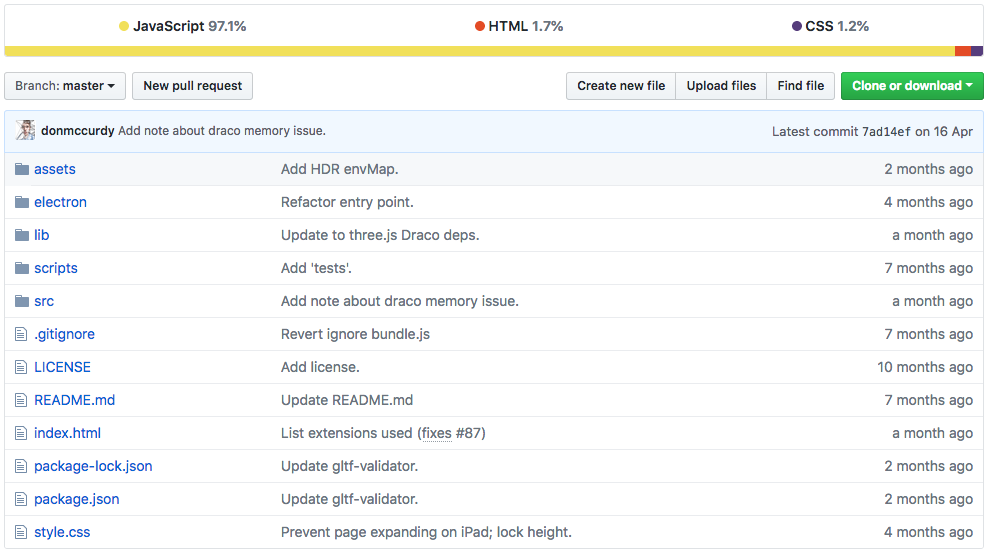
\includegraphics[width=\linewidth]{Figures/three-gltf-viewer-github-preview.png}
    \caption{Statistiques du projet three-gltf-viewer}
    \label{fig:three-gltf-viewer-github-preview}
\end{figure}

Les répertoires situées à la racine nous apprennent l'utilisation du framework Electron https://electronjs.org/.
\subsection{Electron}

\subsection{NodeJS}
Package.json -> Node...

Migration JS -> TS : \url{https://www.typescriptlang.org/docs/handbook/migrating-from-javascript.html}
malheureusement prendrai trop de temps dans le cadre de ce projet. On peut mixer du TS dans du JS mais c'est pas très simple...
Guide pour migrer une app React vers TS : \url{https://github.com/Microsoft/TypeScript-React-Conversion-Guide\#typescript-react-conversion-guide}

Javascript : cours J-L Falcone https://gitlab.unige.ch/courses/jsHepia

\subsection{WebGL}
\textit{WebGL} est une API, basée sur \textit{OpenGL}, servant à afficher des graphiques 2D et 3D dans tout navigateur web compatible\footnote{\url{https://caniuse.com/\#feat=webgl}}, à travers le \textit{canvas} d'\textit{HTML5}. 
Le rendu, au travers du langage \textit{GLSL}, est réalisé par le \textit{GPU}, fournissant ainsi d'excellentes performances. Ces dernières peuvent toutefois être limitées, par exemple sur des ordinateurs équipées d'anciennes cartes graphiques ainsi que les smartphones à la configuration plus modeste.

\textit{WebGL} est développé par le groupe \textit{Khronos}, le même à l'origine du format \textit{glTF} présenté en \ref{sec:glTF}.


\subsection{Three.js}
\textit{Three.js}\footnote{\url{https://threejs.org/}} est une librairie \textit{JavaScript} libre, permettant de créer et afficher des éléments 3D dans un navigateur. Très répandue




\section{Annotations}

\todo{IMG: EXEMPLES D'ANNOTATIONS TEXTE + IMAGE}

Décrire les annotations proposées par Sketchfab : a un titre et une description. Peut aussi être une image.
Principe : en mode édition, double-clic à l'endroit souhaité (point 3d). pour ajouter une annotation. Celle-ci reste liée à la coordonnée choisie, et suit les mouvements appliqués au modèle 3D (p.ex. si on pivote le modèle, alors l'annotation effectue la même transformation).

Choix de technologie :. En gros, on pourrait tout faire en WebGL (REF sur doc WebGL), mais HTML/CSS est bien mieux adapté aux layouts/polices (voir explication en introduction de https://manu.ninja/webgl-three-js-annotations).

\section{Stockage}
Stockage des modèles 3D :
plusieurs solutions sont envisageables. On pourrait utiliser une base de données spécifique aux SIG.
Une première implémentation serait faciliter par un simple stockage des fichiers à l'endroit d'exécution de l'application (sur son serveur p.ex.).


Stockage des annotations :
Format JSON

\subsection{GeoJSON}
\textit{GeoJSON} est un format ouvert,  basé sur JSON, développé pour représenter des caractéristiques géographiques.
Celles-ci incluent les points, les lignes et les polygones ainsi que des sous-ensembles de ces types. À ces éléments, on peut ajouter des attributs.



\section{Hébergement, déploiement}

\subsection{Déploiement en continu avec Heroku}

\textit{Heroku} est une Plateforme \textit{cloud} en tant que service (PaaS) qui offre l'infrastructure nécessaire au déploiement d'applications web. Ainsi, l'équipe de développement peut se concentrer sur le logiciel lui-même sans avoir à gérer la mise en place de serveurs, leur configuration etc.

Parmi les fonctionnalités proposées :
\begin{itemize}
    \item Possibilité de mettre à jour l'application automatiquement au moindre changement dans un \textit{repository} distant, par exemple si le projet est hébergé sur \textit{GitHub},
    \item Scalabilité des processus : en cas de montée en charge (augmentation du nombre de connexions, de traitements à effectuer...), le service offre la possibilité d'allouer des ressources supplémentaires
    \item Isolation : chaque processus est isolé des autres; ainsi si l'un pose problème, le reste du produit n'est pas impacté.
    \item Des logs complets et clairs pour dépanner efficacement son application,
    \item Une documentation vaste, de nombreuses ressources pour démarrer rapidement
\end{itemize}

\textit{Heroku} n'est évidemment pas la seule enterprise à proposer ce genre de services. Citons par exemple \textit{Amazon Web Services (AWS)}, \textit{Windows Azure} ou encore \textit{Google App Engine}.

\textit{Heroku} se démarque quelque peu de la concurrence grâce à la relative rapidité à laquelle on peut mettre en place une première application.


\subsubsection{Problèmes rencontrés}

Heroku considère que l'application se trouve à la racine du dossier.
Si l'application est située dans un sous-répertoire, l'une des possibilités est d'utiliser le module 'subtree' de git, qui permet de créer une sous-arborescence au sein d'un même projet. Ce dernier pourra alors être lié à une branche distincte, dans laquelle il se trouvera à la racine.
\begin{minted}{bash}
    git subtree push --prefix mysubtree origin subtree
\end{minted}

git subtree push --prefix mip-viewer origin heroku

Heroku est un environnement de production (pas de dev). Voir problème rencontré ici :

et commentaire :
Heroku is a production environment. The devDependencies are for packages that are required on your development environment only. Packages that you need to be included in your Heroku slug (including packages required during the slug build phase, such as webpack), need to be in your dependencies, not devDependencies. It is possible that you see people putting webpack in devDependencies for other platforms, but probably not for Heroku. 

et une possible solution étant de créer un script spécifique à Heroku : https://stackoverflow.com/a/42237745/1975002
Avantage : permet de ne pas faire grandir package.json, et d'isoler ce qui concerne Heroku.

Dans mon cas, comme seul le package 'webpack' était concerné, je l'ai "dédoublé" sous dependencies comme suggéré ici : https://stackoverflow.com/a/41973881/1975002

Heroku a pu ainsi faire une première build réussie de l'application. Celle-ci ne fonctionnait malheureusement pas encore correctement (voir \url{https://github.com/MichaelPolla/mip-viewer/issues/5\#issuecomment-390479224}) 

\section{Formats supportés}

On imagine trois cas de figure :

La première possibilité, illustrée en \ref{fig:file-importation-process-native}, est de faire en sorte que l'outil sache lire les fichiers "tels quels", sans effectuer de réelles transformations.
L'avantage est que, pour autant que l'on ait implémenté le support du format de fichier fournit en entrée, celui-ci sera vraisemblablement rendu correctement. C'est un peu le principe des visionneuses d'images classiques, auxquelles on donne les instructions sur "comment lire tel ou tel format de fichier", et qui affichent correctement chaque pixel à l'écran.
Le problème de cette solution est qu'elle nécessite un travail conséquent. Pour qu'elle soit efficace, il faut implémenter bon nombre de formats, et qu'il faut être certain de bien avoir respecter les specifications.

\begin{figure}
    \centering
    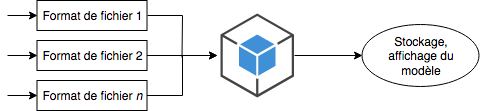
\includegraphics[width=\linewidth]{Figures/file-importation-process-native.png}
    \caption{Cas 1 : support natif des principaux formats}
    \label{fig:file-importation-process-native}
\end{figure}

Une variante est de définir un ou quelques formats principaux, complètement supportés par le logiciel. Si l'utilisateur souhaite importer un modèle stocké sous un format non pris en charge, il devra le convertir manuellement, par exemple à l'aide des fonctions d'exportation du logiciel utilisé pour sa conception.

\begin{figure}
    \centering
    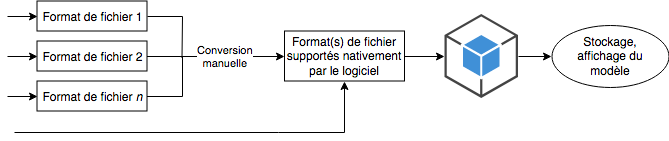
\includegraphics[width=\linewidth]{Figures/file-importation-process-manual-conversion.png}
    \caption{Cas 2 : conversion manuelle vers le(s) format(s) supportés}
    \label{fig:file-importation-process-manual-conversion}
\end{figure}

\begin{figure}
    \centering
    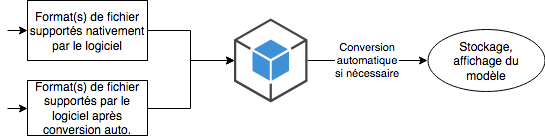
\includegraphics[width=\linewidth]{Figures/file-importation-process-auto-conversion.png}
    \caption{Cas 3 : conversion effectuée par le logiciel, si nécessaire}
    \label{fig:file-importation-process-auto-conversion}
\end{figure}


soit nativement (le logiciel sait lire différents formats), soit en se basant sur un format courant, vers lequel il est relativement aisé de convertir les autres types de fichiers au préalable.

